\documentclass[acmsmall]{acmart}
\bibliographystyle{ACM-Reference-Format}

\usepackage{array}
\usepackage{listings}
\usepackage{tikz}
\usetikzlibrary{positioning}
\usepackage{pgfplots}
\pgfplotsset{compat=1.12}
\usepackage{siunitx}
\usepackage{todonotes}

\title{JuliaPetra: An Implementation of the Petra Object Model in Julia}

\author{Neil Lindquist}
\email{nslindquist@csbsju.edu}

\acmJournal{TOMS}


\newcommand{\snippet}[1]{\lstinline[mathescape]{#1}}


% Julia listings definition
% Definition based on https://tex.stackexchange.com/a/212794/149437
\lstdefinelanguage{Julia}
  {otherkeywords={::},
   keywords=[1]{::,abstract,break,case,catch,const,continue,do,else,elseif,
      end,export,for,function,immutable,import,importall,if,in,
      macro,module,otherwise,quote,return,switch,try,type,typealias,
      using,while,where},
   keywords=[2]{false,true},
   sensitive=true,
   alsoother={$},
   morecomment=[l]\#,
   morecomment=[n]{\#=}{=\#},
   morestring=[s]{"}{"},
   morestring=[m]{'}{'},
}[keywords,comments,strings]

\lstset{
	language         =Julia,
	basicstyle       =\ttfamily\small,
	columns          =fixed,
	numbers          =left,
	numberstyle      =\tiny,
	keywordstyle     ={[1]\bfseries\color{black}},
	keywordstyle     ={[2]\bfseries\color{black}},%{[2]\color{blue}},
	stringstyle      =\color{darkgray},%\color{red},
	commentstyle     =\color{gray},
	showstringspaces =false,
	mathescape
}

\begin{document}
	
	%REVIEW "Distributed algorithms → Self-organization" concept displayed as "self-organization"
	%TODO make sure the concepts represent what I think they do
	\begin{CCSXML}
		<ccs2012>
		<concept>
		<concept_id>10002950.10003714.10003715.10003719</concept_id>
		<concept_desc>Mathematics of computing~Computations on matrices</concept_desc>
		<concept_significance>500</concept_significance>
		</concept>
		<concept>
		<concept_id>10002950.10003705</concept_id>
		<concept_desc>Mathematics of computing~Mathematical software</concept_desc>
		<concept_significance>100</concept_significance>
		</concept>
		<concept>
		<concept_id>10010147.10010148.10010149.10010158</concept_id>
		<concept_desc>Computing methodologies~Linear algebra algorithms</concept_desc>
		<concept_significance>500</concept_significance>
		</concept>
		<concept>
		<concept_id>10010147.10010919.10010172.10003824</concept_id>
		<concept_desc>Computing methodologies~Self-organization</concept_desc>
		<concept_significance>100</concept_significance>
		</concept>
		</ccs2012>
	\end{CCSXML}
	
	\ccsdesc[500]{Mathematics of computing~Computations on matrices}
	\ccsdesc[100]{Mathematics of computing~Mathematical software}
	\ccsdesc[500]{Computing methodologies~Linear algebra algorithms}
	\ccsdesc[100]{Computing methodologies~Self-organization}
	
	\begin{abstract}
		JuliaPetra provides linear algebra data structures that are commonly used in large scale, linear solver algorithms.
		The data structures in JuliaPetra focus on vectors and sparse matrices, in both serial and
		distributed, parallel environments.
		The library is written in Julia, a high level programming language with comparable performance to C and Fortran.
		JuliaPetra performs as fast as Epetra, an equivalent C++ library, and faster than DistributedArrays.jl, a Julia
		library for distributed computations on arrays.
	\end{abstract}
	
	\maketitle
	
	\section{Introduction}
	
	JuliaPetra is an implementation of the Petra object model in Julia.
	The Petra object model is the design used in Trilinos for objects commonly used by linear solver algorithms~\cite{Heroux:2005:Trilinos}.
	Petra libraries provide parallel, distributed matrices, vectors, and graphs for other packages to use.
	By providing a set of interfaces for basic linear algebra structures, Petra libraries provide a way
	to develop packages for these types of distributed algorithms that can interact and build on each other.
	The Petra object model has previously been implemented in both C++ and Java.
	Like other implementations of the Petra object model, JuliaPetra provides the ability to do basic linear algebra computations, including dot products, vector norms, and sparse matrix-vector multiplications.
	
	Julia is a programing language that uses just in time compiling and powerful type inferencing
	to obtain the speed of a statically compiled programing language with the productivity of an
	interpreted programing language~\cite{Bezanson:2017:FreshApproach}.
	By providing speed comparable to that of Fortran or C, Julia is a candidate for doing large scale,
	high performance computations.
	The Celeste project is an example of large scale computations in Julia,
	using 8,192 cores of the Cori Supercomputer
	at Lawrence Berkeley National Laboratory~\cite{Bezanson:2017:FreshApproach}.
	
	\section{The Petra Object Model}
	
	\todo[inline]{
		A general discussion of the Petra Object model, along with class diagrams.
	}
	
	\section{Design of JuliaPetra}
	
	The design of JuliaPetra follows closely with that of the C++ implementations of the
	Petra object model, Epetra and Tpetra.
	Like Epetra and Tpetra, JuliaPetra uses MPI and Single-Program-Multiple-Data as its base parallel model.
	The API is split into three main layers of abstraction, the communication layer, the problem distribution layer, and the data structures layer.
	
	The first level of abstraction handles actual communication between processes.
	The \snippet{Comm} and \snippet{Distributor} types provide a low level interface to support different communication methods.
	Because all interprocess communication is done through these objects, new communication systems can be implemented without affected the objects built on top of the communication layer.
	There are two existing implementations of this layer, a serial implementation, with a trivial implementation, and an MPI implementation, built on MPI.jl~\cite{Github:MPI}.
	This communication layer provides the abstraction to build Single-Program-Multiple-Data logic without regard for the underlying communication implementation.
	
	The next layer of abstraction manages how the problem is distributed across processes.
	The \snippet{BlockMap}, \snippet{Directory}, \snippet{Import} and \snippet{Export}
	types handle the distribution of the problem across the processes.
	\snippet{BlockMap} and \snippet{Directory} manage which process the various parts of
	the problem are located.
	\snippet{Import} and \snippet{Export} contain the logic behind redistributing
	the problem among the processes.
	The \snippet{SrcDistObject} and \snippet{DistObject} interfaces provide a connection between
	the redistributing logic and the data structures themselves.
	This provides an abstraction on which the distributed data structures can build.
	
	The linear algebra objects are built on top of the abstractions provided by the problem distribution layer.
	JuliaPetra has two main linear algebra types.
	The first type is the abstract type \snippet{MultiVector} which holds one or more vectors.
	This type is implemented by \snippet{DenseMultiVector} which stores dense vectors.
	The second type is the \snippet{Operator} interface which is implemented by types that provide a
	\(y \gets \alpha\cdot A(x) + \beta\cdot y\) operation, where \(\alpha\) and \(\beta\) are scalars,
	\(x\) and \(y\) are vectors and \(A\) is the operator.
	The abstract type \snippet{RowMatrix}, which stores sparse matrices accessed by rows,
	supports this interface by multiplying the matrix on the left of \(x\).
	\snippet{RowGraph} is an additionally type used to represent the sparsity pattern of a \snippet{RowMatrix}.
	Both \snippet{RowMatrix} and \snippet{RowGraph} have concrete implementations based on
	compressed sparse row format, \snippet{CSRMatrix} and \snippet{CSRGraph}, respectively.
	Julia's \snippet{AbstractArray} is subtyped by both the \snippet{MultiVector}
	and \snippet{RowMatrix} types to allow existing Julia code to interact with data in JuliaPetra objects.
	
	\begin{figure}
		%name, type, location
		\newcommand{\typeNode} [3]{\node[#2] (#1) [#3] {\snippet{#1}};}
		\newcommand{\explicitInheritance}[2]{\draw[->] (#1.south) -- (#2);}
		\newcommand{\implicitInheritance}[2]{\draw[dashed,->] (#1.south) -- (#2);}
		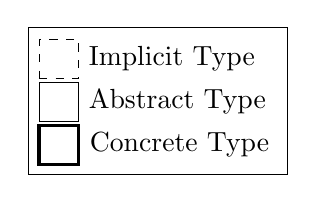
\begin{tikzpicture}[
		ImplicitInterface/.style={rectangle, draw=black, dashed, minimum size=5mm},
		ExplicitInterface/.style={rectangle, draw=black, minimum size=5mm},
		ConcreteType/.style={rectangle, draw=black, very thick, minimum size=5mm}
		]
		
		\typeNode{Comm}{ExplicitInterface}{}
		
		\typeNode{MPIComm}{ConcreteType}{below=.75cm of Comm}
		\explicitInheritance{Comm}{MPIComm.north}
		
		\typeNode{SerialComm}{ConcreteType}{right=.25cm of MPIComm}
		\explicitInheritance{Comm}{SerialComm.north}
		
		\typeNode{LocalComm}{ConcreteType}{left=.25cm of MPIComm}
		\explicitInheritance{Comm}{LocalComm.north}
		
		\typeNode{Distributor}{ExplicitInterface}{left=5.1cm of Comm}
		
		\typeNode{SerialDistributor}{ConcreteType}{below right=.75cm and -1cm of Distributor}
		\explicitInheritance{Distributor}{SerialDistributor.north}
		
		\typeNode{MPIDistributor}{ConcreteType}{left=.25cm of SerialDistributor}
		\explicitInheritance{Distributor}{MPIDistributor.north}
		
		
		
		\typeNode{Directory}{ExplicitInterface}{below right=.75cm and -1.25cm of MPIDistributor}
		
		\typeNode{BasicDirectory}{ConcreteType}{below=.75cm of Directory}
		\explicitInheritance{Directory}{BasicDirectory.north}
		
		\typeNode{BlockMap}{ConcreteType}{right=of Directory}
		
		\typeNode{Import}{ConcreteType}{right=of BlockMap}
		
		\typeNode{Export}{ConcreteType}{right=of Import}
		
		
		
		\typeNode{SrcDistObject}{ImplicitInterface}{below left=.75cm and -.9cm of Export}
		
		\typeNode{DistObject}{ImplicitInterface}{below=.75cm of SrcDistObject}
		\implicitInheritance{SrcDistObject}{DistObject.north}
		
		\typeNode{Operator}{ImplicitInterface}{left=of DistObject}
		
		\typeNode{AbstractArray}{ExplicitInterface}{left=of Operator}
		
		\typeNode{MultiVector}{ExplicitInterface}{below=of AbstractArray}
		\implicitInheritance{DistObject}{MultiVector.north east}
		\explicitInheritance{AbstractArray}{MultiVector.north}
		
		\typeNode{DenseMultiVector}{ConcreteType}{below=.75cm of MultiVector}
		\explicitInheritance{MultiVector}{DenseMultiVector.north}
		
		\typeNode{RowMatrix}{ExplicitInterface}{below=of Operator}
		\implicitInheritance{DistObject}{RowMatrix.north east}
		\implicitInheritance{Operator}{RowMatrix.north}
		\explicitInheritance{AbstractArray}{RowMatrix.north west}
		
		\typeNode{RowGraph}{ExplicitInterface}{below=of DistObject}
		\implicitInheritance{DistObject}{RowGraph.north}
		
		\typeNode{CSRMatrix}{ConcreteType}{below=.75cm of RowMatrix}
		\explicitInheritance{RowMatrix}{CSRMatrix.north}
		
		\typeNode{CSRGraph}{ConcreteType}{below=.75cm of RowGraph}
		\explicitInheritance{RowGraph}{CSRGraph.north}
		
		\matrix [draw,below=.25cm] at (current bounding box.south) {
			\node[ImplicitInterface,label=right:Implicit Type] {}; \\
			\node[ExplicitInterface,label=right:Abstract Type] {}; \\
			\node[ConcreteType,label=right:Concrete Type] {}; \\
		};
		
		\end{tikzpicture}
		\Description{The type hiearchy of JuliaPetra.  The relationships of note are how \snippet{MultiVector}, \snippet{RowMatrix} and \snippet{RowGraph} implement the implicit type \snippet{DistObject} and how both \snippet{MultiVector} and \snippet{RowMatrix} are subtypes of Julia's \snippet{AbstracyArray}.}
		\caption{Type Hierarchy of JuliaPetra.}
		\label{fig:type-hierarchy}
	\end{figure}
	
	The type hierarchy in JuliaPetra is limited by the fact that types in Julia are restricted to a single supertype.
	Interacting with existing code as a 2-dimensional array requires being a subtype of \snippet{AbstractArray}.
	So, the other interfaces for the data structures are not explicit types,
	but simply contracts promised in the documentation.
	These implicit interfaces include \snippet{Operator}, \snippet{SrcDistObject}
	and \snippet{DistObject}.
	%TODO consider discussing the vagueness of the definition of (Src)DistObject
	So, any methods that use one of those types accepts an object of any type
	and the documentation specifies the methods that must be implemented.
	Figure~\ref{fig:type-hierarchy} shows the full type hierarchy.
	
	\section{JuliaPetra Syntax}
	
	For an example usage of JuliaPetra, Listing~\ref{lst:JP-PCG} contains an implementation of the preconditioned conjugate gradient implemented with JuliaPetra.
	Note that because vectors are stored in groups as \snippet{MultiVector}s, the implementations support solving multiple right hand sides at the same time.
	This implementation provides two functions: one that updates \snippet{x} in place, \snippet{conjugate_gradient!}; and one that copies \snippet{x}, \snippet{conjugate_gradient}.
	Note that function names ending in exclamation marks is merely Julia convention to warn the user that an input is mutated in the function call.
	Each function takes four mandatory arguments: \snippet{x}, the initial guess; \snippet{A}, the linear operator being solved; \snippet{b}, the right hand side; and \snippet{Minv}, the preconditioning function.
	Additionally, there are two keyword arguments: \snippet{niters}, the maximum number of iterations; and \snippet{tol}, the target tolerance.
	
	\begin{lstlisting}[float,
						caption=Preconditioned Conjugate Gradient in JuliaPetra,
						label=lst:JP-PCG,
						escapechar=|]
function conjugate_gradient(x::MultiVector{Data, GID, PID, LID}, A,
        b::MultiVector{Data, GID, PID, LID}, Minv;
        niters = 100, tol = 1e-6) where {Data, GID, PID, LID}
    x = copy(x)
    conjugate_gradient!(x, A, b, Minv; niters=niters, tol=tol)
    x
end

function conjugate_gradient!(x::MultiVector{Data, GID, PID, LID}, A,
        b::MultiVector{Data, GID, PID, LID}, Minv;
        niters = 100, tol = 1e-6) where {Data, GID, PID, LID}
    r = apply(b, A, x, Data(-1), Data(1)) # r = -Ax + b
    z = MultiVector{Data}(getMap(x), numVectors(x), false)
    apply!(z, Minv, r) # z = Minv*r
    p = copy(z)

    Ap = MultiVector{Data}(getMap(b), numVectors(b), false)

    r$\,^t$z = r$\,\mathtt{\boldsymbol{\cdot}}\,$z # = dot(r, z) |\label{line:dot}\label{line:^t}|

    for k in 1:niters
        apply!(Ap, A, p)
        pAp = p$\,\mathtt{\boldsymbol{\cdot}}\,$Ap |\label{line:dot2}|
        $\alpha$ = r$\,^t$z ./ pAp |\label{line:alpha}|

        @. x = x + $\alpha$ * p |\label{line:line-broadcast}|
        @. r = r - $\alpha$ * Ap

        apply!(z, Minv, r)

        r$\,^t$z_old = r$\,^t$z
        r$\,^t$z = r$\,\mathtt{\boldsymbol{\cdot}}\,$z |\label{line:dot3}|
        if !any(sqrt.(rtz) .> tol) |\label{line:operator-broadcast}|
            break
        end
        $\beta$ = r$\,^t$z/r$\,^t$z_old |\label{line:beta}|
        @. p = z + $\beta$ * p
    end
    x
end
	\end{lstlisting}
	
	As the example shows, Julia's syntax is similar to that of Fortran and MATLAB.
	Furthermore, but not show, Julia uses one based indices and supports multidimensional arrays (including slices)~\cite{Bezanson:2017:FreshApproach}.
	Julia also supports syntactic macros that process the abstract syntax tree of their arguments, like macros in lisp-like languages (and unlike token based macros in C and C++).
	
	
	Julia has strong support for Unicode characters~\cite{Bezanson:2017:FreshApproach}.
	First, note how both \(\alpha\) and \(\beta\) are used for variable names, as declared on lines~\ref{line:alpha} and~\ref{line:beta}, respectively.
	In addition to supporting Greek characters, Julia supports letter exponents in variable names.
	For example, on line~\ref{line:^t} the value of \(r^tz\) is stored in the variable \texttt{r$\,^t$z}. % using \texttt because \lstinline isn't behaving with mathmode
	Finally, note the use of a dot symbol for the dot product, as shown on lines~\ref{line:dot}.
	To allow for these and other characters, Julia editors, including the console interface, provide latex like commands to type many Unicode characters.
	For example, \texttt{\textbackslash alpha} followed by the tab key generates \(\alpha\).
	Additionally, Julia can be used with just ASCII characters.
	Operations like dot products have ASCII function name equivalents, as shown in line~\ref{line:dot}.
	
	Another convenience Julia provides and JuliaPetra takes advantage of is the broadcast operator~\cite{Bezanson:2017:FreshApproach}.
	Examples can be seen in lines~\ref{line:line-broadcast} and~\ref{line:operator-broadcast}.
	The broadcast operator takes operations on container objects and applies them to each element in the container, allowing any function to be applied element-wise.
	Additionally, Julia automatically fuses the loops where able, so, for example, line~\ref{line:line-broadcast} will be computed with only a single loop and no intermediate vectors.
	Julia provides two, interchangeable ways to broadcast operations and functions.
	Each function call can broadcast individually, as shown on line~\ref{line:operator-broadcast}, or each function in a line can be broadcast, as shown on line~\ref{line:line-broadcast}.
	Note that JuliaPetra works with multivectors instead of plain vectors, so operations like dot products return array with each of the respective results.
	These functions and JuliaPetra's broadcasting are implemented so that each result is seamlessly able to be applied to the appropriate vector in the set.
	
	\section{Optimizations of JuliaPetra}
	%This is to give insight on best practices for people who don't look at the general Julia discussions
	%Talk about the "story" of improving the code and how optimizations improved performance.
	
	There were a lot of optimizations used to optimize JuliaPetra, many of which are standard advice for optimizing Julia, such as type stability, or for optimization in general, such as accessing arrays in memory order.
	The only major, unusual optimization was using \snippet{Ptr} objects to pass views of arrays to reduce allocation and garbage collection.
	
	The main improvements to performance in JuliaPetra came from improving type stability.
	Type stability is where the compiler can inference the types of all values.
	This allows the compiler to fully inline function calls, especially arithmetic and array operations.
	Because Julia is designed to support both slower, type unstable code and faster, type stable code,
	unlike C++ which is restricted to type stable code, some effort needs to be put into verifying
	type stability of performance critical code~\cite{Bezanson:2017:FreshApproach}.
	%REVIEW mention that this is standard Julia advice?
	Removing type instabilities from performance critical sections of JuliaPetra improved performance
	by a few orders of magnitude.
	The \snippet{code_warntype} function was a valuable tool in finding type instabilities.
	Due to \snippet{code_warntype} requiring manual inspection, the TypeStability.jl library was created
	based on \snippet{code_warntype} to automatic type stability checks~\cite{Github:TypeStability.jl}.
	
	Another notable optimization came from using \snippet{Ptr} objects to pass views of arrays.
	Because Julia is a garbage collected language, most objects in Julia must be allocated on the heap,
	then garbage collected when they are no longer used.
	However, certain objects, such as integers and floating point numbers can be allocated on the stack,
	so they avoid needing garbage collection.
	%needs some citations here
	So, by passing \snippet{Ptr} objects, which can be stack allocated,
	instead of \snippet{SubArray} objects, which must be heap allocated,
	the heap allocations and garbage collection can be greatly reduced in some performance critical sections
	However, this prevents use of higher level interfaces that Julia normally provides,
	such as the array length being stored with the array its self.
	This had much less of a performance increase that improving type stability,
	however, it is not a standard optimization for Julia, so it deserved mention.
	
	Other common and minor optimizations were also made.
	These optimizations include skipping unnecessary bounds checks
	and ensuring arrays data was accessed in the order it is stored in memory.
	Additionally, function calls in frequently used loops were replaced with specialized, inlined versions that consider the context of the calling method and avoid using generalized methods that produce extra computations.
	%REVIEW should I go into more detail on the specific example (getting a row in SpMV)
	
	\section{Comparisons with Other Distributed Libraries}
	
	To determine the quality of JuliaPetra as a distributed linear algebra library, it is compared to two existing libraries, Epetra and DistributedArrays.jl.
	JuliaPetra is close to the former, as it was implemented partially based on Epetra.
	It varies much more from the latter; JuliaPetra has much better performance but deviates from some Julia conventions.
	
	\subsection{Comparison with Epetra}
	
	Epetra is the base implementation of the Petra object model,
	written in a stable subset of C++~\cite{Heroux:2005:Trilinos}.
	Because Epetra was used as a template for implementing JuliaPetra,
	the APIs for JuliaPetra are similar to those for Epetra.
	The similarities between JuliaPetra and Epetra can be seen in how similar the respective implementations
	of the power method are.
	The differences in features between the implementation languages result in differences
	between JuliaPetra's and Epetra's APIs.
	For example, JuliaPetra takes advantage of higher level structures
	such as type templating and thrown exceptions.
	
	JuliaPetra can achieve the same performance as Epetra on large instances of the power method, as shown in Table~\ref{tab:timing-results}.
	Since Julia uses just in time compiling, the JuliaPetra power method has extra startup costs compared to
	the Epetra version. However, since each specialized method needs to be compiled only once,
	this is a fixed cost during the first evaluation.
	Additionally, JuliaPetra uses runtime dispatch in a few locations, such as with
	\snippet{Comm} objects, which adds additional overhead compared to Epetra.
	
	\subsection{Comparison with DistributedArrays.jl}
	
	DistributedArrays.jl is a similar library to JuliaPetra that supports
	distributed arrays in parallel environments~\cite{Github:DA}.
	It uses Julia's built in fork-and-join model for parallelism~\cite{Bezanson:2017:FreshApproach}.
	DistributedArrays.jl offers several of usability advantages over JuliaPetra, however, it is not able to match the speed of JuliaPetra.
	
	DistributedArrays.jl has advantages over JuliaPetra because it is better designed to function with
	existing Julia code.
	For example, it is built around the standard models of parallelization and arrays in Julia.
	Another advantage is that DistributedArrays.jl uses an instance of \snippet{AbstractArray}
	for a process's local storage, this allows automatic support for different array structures.
	Finally, by keeping the program logic on the master process, DistributedArrays.jl can be used to
	do distributed computations while using Julia's read-eval-print loop.
	
	However, DistributedArrays.jl is performs much worse for the sparse operations used in the comparison timings.
	This difference in performance likely stems from the fact that DistributedArrays.jl is optimized towards dense matrix operations, resulting in unnecessary communication and computation when working with sparse matrices.
	A Julia 0.6.0 version of DistributedArrays.jl was modified to be more conducive to sparse matrix operations, but that implementation was neither able to match the performance of JuliaPetra nor updated to the Julia 1.0 compatible version of DistributedArrays.jl.
	
	\subsection{Timing Results}
	
	\begin{table}
		\caption{Timing results of various power method implementations.  All times are in seconds.}
		\label{tab:timing-results}
		\begin{tabular}{|c c|S|S|S||S|}
			\hline
			\multicolumn{2}{|c|}{Equations Per Process}
			& {JuliaPetra}
			& {Epetra}
			& \multicolumn{1}{m{1.8cm}||}{Distributed\-Arrays.jl}
			& \multicolumn{1}{m{1.75cm}|}{JuliaPetra \(\div\) Epetra}\\
			\hline
			\multicolumn{6}{|l|}{4 Processes}\\
			
			\hline
			100,000			&Mean    & 0.22514 & 0.19244 & 124.322 & 1.16988 \\
			equations		&Minimum & 0.22183 & 0.18437 & 123.324 & 1.20509 \\
							&Maximum & 0.22747 & 0.22145 & 126.464 & 1.02721 \\
			\hline
			1,000,000		&Mean    & 2.76858 & 2.35595 & 1149.26 & 1.17515 \\
			equations		&Minimum & 2.75613 & 2.35066 & 1144.52 & 1.12492 \\
							&Maximum & 2.78917 & 2.36304 & 1162.54 & 1.18033 \\
			\hline
			10,000,000		&Mean    & 30.8755 & 24.7034 & {-} & 1.24985 \\
			equations		&Minimum & 30.6740 & 24.6805 & {-} & 1.24284 \\
							&Maximum & 31.1139 & 24.7140 & {-} & 1.25896 \\
			\hline
			\multicolumn{6}{|l|}{16 Processes}\\
			\hline
			100,000			&Mean    & 0.53649 & 0.50143 & 2569.82 & 1.06990 \\
			equations		&Minimum & 0.53408 & 0.49653 & 2525.37 & 1.07562 \\
							&Maximum & 0.53741 & 0.50376 & 2713.96 & 1.06680 \\
			\hline
			
			1,000,000		&Mean    & 7.51502 & 7.40649 & {-} & 1.01465 \\
			equations		&Minimum & 7.49275 & 7.40309 & {-} & 1.01211 \\
							&Maximum & 7.54793 & 7.41002 & {-} & 1.01861 \\
			\hline
			10,000,000		&Mean    & 74.2079 & 73.9740 & {-} & 1.00316 \\
			equations		&Minimum & 74.0943 & 73.9240 & {-} & 1.00230 \\
							&Maximum & 74.2893 & 74.0402 & {-} & 1.00336 \\
			\hline
			\multicolumn{6}{|l|}{20 Processes}\\
			\hline
			100,000			&Mean    & 0.77256 & 0.70583 & {-} & 1.09454 \\
			equations		&Minimum & 0.73311 & 0.70270 & {-} & 1.04328 \\
							&Maximum & 0.80217 & 0.71200 & {-} & 1.12663 \\
			\hline
			1,000,000		&Mean    & 9.89883 & 9.22033 & {-} & 1.07359 \\
			equations		&Minimum & 9.85269 & 9.21825 & {-} & 1.06882 \\
							&Maximum & 9.97940 & 9.22443 & {-} & 1.08184 \\
			\hline
			10,000,000		&Mean    & 97.4143 & 92.0917 & {-} & 1.05780 \\
			equations		&Minimum & 96.9243 & 91.9722 & {-} & 1.05384 \\
							&Maximum & 97.9733 & 92.1464 & {-} & 1.06324 \\
			\hline
		\end{tabular}
	\end{table}
	
	\todo[inline]{
		The timing results could be a bit confusing to the reader.  It would be worth mentioning specifically what the total number of equations is, at least in the description.  Better notes on speedups could improve it.  Also, it would be good to get some timing results from something beyond a tridiagonal matrix.
	}
	
	As can be seen in Table~\ref{tab:timing-results}, JuliaPetra is close to the performance of Epetra, except when only using a few processes.
	Additionally, JuliaPetra significantly outperforms DistributedArrays.jl.
	Note that the last column shows the ratio of the JuliaPetra time over the Epetra time; in other words, a higher ratio indicates that the same problem will take longer to solve using JuliaPetra compared to Epetra.
	Additionally, the number of iterations was consistent between all problems, meaning the number of operations completed is only a function of number of processes and local problem size.
	The sizes were chosen to test how the libraries respond to different local workloads.
	
	Figure~\ref{fig:result-numProcs} compares the performance of JuliaPetra and Epetra over a varying number of processes for a fixed problem size.
	Note that for fewer processes, JuliaPetra under performs Epetra.
	However, as the number of processes increases, JuliaPetra approaches the performance of Epetra.
	Although, when all 20 cores of the process are used JuliaPetra has a slight drop in performance.
	The reason for this has not been determined but is suspected to be related to Julia relying more heavily on cache and the operating system not having extra cores to run its other processes on.
	Because JuliaPetra performs closer to Epetra when more processes are present, it seems that JuliaPetra may be slower for the actual computations, but the communication for larger problems overcomes the difference or is more efficient in JuliaPetra.
	
	\begin{figure}
		\centering
		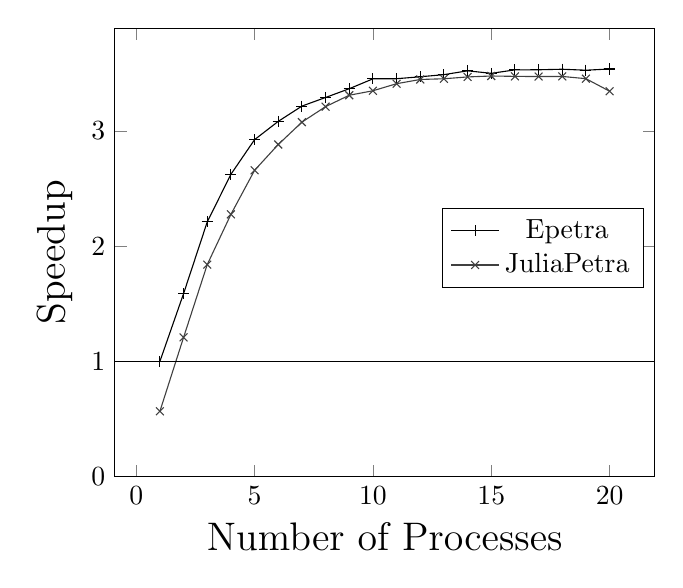
\begin{tikzpicture}
			\begin{axis}[
				xlabel = {\Large Number of Processes},
				ylabel style = {align=center},
				ylabel = {\Large Speedup},
				ymin = 0,
				legend style={at={(0.98,0.6)}}
			]
				\addplot[color=black,mark=+] coordinates{(1, 1) (2, 1.5883416) (3, 2.210738) (4,2.6240833) (5, 2.924896) (6,3.083557) (7, 3.216142) (8,3.290998) (9,3.36702) (10, 3.452862) (11,3.45405) (12,3.470708) (13,3.489314) (14,3.52233) (15, 3.500694) (16,3.53057) (17,3.53162) (18,3.536203) (19, 3.5278034) (20, 3.538395)};
				\addlegendentry{Epetra}
				\addplot[color=darkgray,mark=x] coordinates{(1, 0.5667807) (2, 1.208247) (3, 1.8400692) (4,2.276446) (5, 2.658824) (6,2.882781) (7, 3.0769025) (8,3.21155) (9,3.31040) (10, 3.349281) (11,3.410606) (12,3.447333) (13,3.453482) (14,3.4693506) (15, 3.4774509) (16,3.474327) (17,3.472608) (18,3.473677) (19, 3.4541359) (20, 3.345339)};
				\addlegendentry{JuliaPetra}
				\draw (axis cs:-1,1) -- (axis cs:25,1);
			\end{axis}
		\end{tikzpicture}
		\caption{Speedup over a single process of Epetra (with an MPI communicator) for \(10^7\) rows.}
		\label{fig:result-numProcs}
		\Description{
			A comparison of the performance of Epetra and JuliaPetra for 1 to 20 processes.
			JuliaPetra noticably underperforms Epetra for low numbers of processes, but roughly matches the performance of Epetra when the number of processes is in the double digits.
		}
	\end{figure}

	The timings come from implementations of the power method for finding the largest eigenvalue of a matrix
	\cite{Gu:2000:PowerMethod}.
	Epetra's \texttt{petra\_power\_method} example is used as the Epetra implementation and the other implementations are translations of that code~\cite{Heroux:2005:Trilinos}.
	This tests the performance of vector dot product, vector L2-norm and sparse matrix-vector multiplication functionalities.
	The matrices used were various sizes of symmetric tridiagonal matrices, with the diagonal consisting of 2's
	and the off diagonals containing -1's, that were distributed over different numbers of processes.
	Each combination of implementation, problem size, and number of processes was run five times and the average, minimum and maximum are presented.
	All implementations were run once before collecting the timings, to ensure all Julia code was
	compiled before the timing started.
	Additionally, the setup for the problems were not counted as part of the times.
	Finally, only the MPI based communicator was used for the Petra implementations.
	Note that the DistributedArrays.jl implementation took over an hour to find the eigenvalue for some problem sizes.
	Given the timings produced by the Petra implementations, these problems were not run to completion and left without a time on the table.
	
	The MPI implementation was MPICH version 3.2 with TCP used for all inter-process communication, with MPI.jl version 0.7.0 wrapping MPI for JuliaPetra.
	The \texttt{mpiexec} command was used to start the MPI processes with the \texttt{-bind-to core} and \texttt{-map-by core} flags.
	The Julia tests were run with the Julia v1.0.0 precompiled binary for Linux with the \texttt{-O3} flag enabled at run time.
	Version 0.5.1 of DistributedArrays.jl was used.
	The Epetra tests were compiled with GCC 4.8.5, the \texttt{-O3} flag and Trilinos 12.10.1.
	Tests were run on a Red Hat Enterprise Linux Workstation, version 7.3,
	with a 20 core Intel E5-2698 v4 CPU.
	
	\section{Conclusion}
	
	JuliaPetra is an implementation of the Petra object model in the Julia programming language.
	So, it provides an interface for distributed solver algorithms to interact with and build on each other.
	Additionally, by performing at the same speeds as Epetra,
	it allows Julia to compete with C++ for these types of high performance computations.
	This implementation demonstrates that Julia is a suitable candidate for these types of large scale, high performance, distributed codes.
	
	%REVIEW are there other things that should be discussed in the conclusion
	%It feels pretty short
	
	\bibliography{bibliography}
\end{document}
